\documentclass[11pt]{elsarticle}

\usepackage[acronym]{glossaries}
\usepackage{paralist}
\usepackage{amsmath}
\usepackage{amssymb}
\usepackage{booktabs}
\usepackage{graphicx}
\usepackage{multirow}
\usepackage{color, colortbl}

\definecolor{Gray}{gray}{0.9}
\usepackage[table,xcdraw]{xcolor}
\usepackage[font=small]{caption}
\setlength{\abovecaptionskip}{0pt plus 3pt minus 2pt} 
\usepackage[spanish, english]{babel} 
\DeclareMathOperator*{\argmax}{arg\,max}
\DeclareMathOperator*{\argmin}{arg\,min}
\usepackage{setspace}  
\usepackage{tikz}
\usetikzlibrary{arrows,petri,topaths,quotes}
\tikzset{invisible/.style={minimum width=0mm,inner sep=0mm,outer sep=0mm}}
\usepackage{subcaption} 
\definecolor{A}{gray}{0.95}
\definecolor{B}{gray}{0.85}
\definecolor{C}{gray}{0.75}
\definecolor{D}{gray}{0.65}
\definecolor{E}{gray}{0.55}
\definecolor{F}{gray}{0.45}
\definecolor{G}{gray}{0.35}
\definecolor{H}{gray}{0.25}
\definecolor{I}{gray}{0.15}
\definecolor{CITE}{HTML}{0571B0}
\definecolor{greencolor}{HTML}{029386}
\definecolor{bluecolor}{RGB}{8,96,168}
\usepackage{amsthm}
\theoremstyle{plain}
\newtheorem{theorem}{Theorem}
\newtheorem{corollary}{Corollary}
\newtheorem{lemma}{Lemma}
\newtheorem{proposition}{Proposition}
\newtheorem{definition}{Definition}
\usepackage{tabularx}
\usepackage{url}
\AtBeginDocument{\hypersetup{citecolor=CITE, linkcolor=CITE, citecolor=CITE, urlcolor=CITE}}
\usepackage{float}
\usepackage{makecell}
\newcommand{\blue}[1]{\textcolor{blue}{#1}}
\newcommand{\red}[1]{\textcolor{red}{#1}}
\usepackage{color, colortbl}
\allowdisplaybreaks
\usepackage{verbatim}
\usepackage{listings}
\lstset{
  basicstyle=\ttfamily,
  breaklines=true,
  breakatwhitespace=true,
  columns=fullflexible
}
\usepackage[]{acronym}
\usepackage{lipsum}
\usepackage{amsmath}
\usepackage{glossaries}
\usepackage[toc]{appendix} % Appendices TOC
\setcounter{tocdepth}{2} % So sections and subsections appear in the TOC
\usepackage{algorithm}
\usepackage{algpseudocode}
\usepackage{amsmath}
\usepackage{array}
\usepackage{booktabs}
\usepackage{amsmath}
\usepackage{amsfonts}
\usepackage{mathtools}
\usepackage[left=1in,right=1in,top=1in,bottom=1in,margin=1in]{geometry} % Consolidated geometry options
\usepackage{etoc} % For the Appendices mini TOC
\usepackage[colorlinks = true, linkcolor=CITE, citecolor=CITE, urlcolor=CITE]{hyperref}
\usepackage[T1]{fontenc}
\usepackage{lmodern}
\usepackage{microtype}
\renewcommand{\sectionautorefname}{Section}
\renewcommand{\subsectionautorefname}{Subsection}
\renewcommand{\subsubsectionautorefname}{Subsubsection}

\makeatletter
\def\ps@pprintTitle{%
  \let\@oddhead\@empty
  \let\@evenhead\@empty
  \def\@oddfoot{\reset@font\hfil\thepage\hfil}
  \let\@evenfoot\@oddfoot
}
\makeatother

\begin{document}

% \newpageafter{author}

\begin{frontmatter}

\title{Designing Multi-Compartment Last-Mile Vehicle Fleets: An Open-Source Matheuristic}

% \author[ERIC-UTDT]{Eric Kohan}
% \author[FABRICIO-UFMG]{Fabricio Torres}
% \author[UNAB-Address,MIT-Address]{Victor Silva-Febre}
% \author[PUCV-Address,MIT-Address]{J.C. Pina-Pardo\corref{mycorrespondingauthor}}
% \cortext[mycorrespondingauthor]{Corresponding author}
% \ead{juan.pina@pucv.cl, juanpina@mit.edu}

% \address[ERIC-UTDT]{Universidad Torcuato Di Tella, Buenos Aires, Argentina}
% \address[FABRICIO-UFMG]{Universidade Federal de Minas Gerais, Belo Horizonte, Brazil}
% \address[UNAB-Address]{Universidad Nacional Andrés Bello, Santiago, Chile}
% \address[MIT-Address]{Massachusetts Institute of Technology, Cambridge, USA}
% \address[PUCV-Address]{Pontificia Universidad Católica de Valparaíso, Valparaíso, Chile}

\onehalfspacing

% \begin{highlights}
% \item We study a fleet size and mix problem with heterogeneous multi-compartment vehicles.
% \item We propose a novel matheuristic approach based on a cluster-first, fleet design-second scheme.
% \item We present \textsc{FleetMix}, a spec-driven, open-source implementation of our matheuristic.
% \item We show the effectiveness of \textsc{FleetMix} compared to existing solution approaches.
% \item We derive several managerial insights for a real-world case study.
% \end{highlights}

\begin{abstract}	
Urban food distributors are increasingly relying on flexible, multi-compartment vehicle fleets to handle diverse product mixes and challenging urban environments. While recent research on multi-compartment vehicle routing problems has explored a range of heuristics and constraints, to our knowledge, none has directly addressed fleet size and mix optimization for heterogeneous vehicles with flexible compartments in food distribution systems. Motivated by our collaboration with a major food distributor operating in Colombia, we close this practical and methodological gap by proposing a novel cluster-first, fleet design-second matheuristic approach that quickly produces cost-effective fleet size and mix solutions. 
To support practitioners and researchers in applying and replicating our results, we make our matheuristic publicly available through \textsc{FleetMix}, an open-source Python package freely available under the MIT license and distributed via PyPI.
We show the effectiveness of \textsc{FleetMix} in finding high-quality solutions compared to existing solution approaches on available benchmark instances. Based on a real-world case study from our industry partner, which serves hundreds of customers daily, we also show the value of utilizing multi-compartment vehicles to reduce fleet sizes and total logistics costs.
\end{abstract} 

\begin{keyword}
fleet design \sep multi-compartment \sep matheuristic \sep open-source Python package \sep last mile
\end{keyword}
	
\end{frontmatter}

\setlength{\parskip}{1.5mm}
\onehalfspacing

\section{Introduction} \label{sec:introduction}

The growing expansion of the food industry has drawn increasing attention to food safety and quality management during production, storage, and transportation \citep{hsiao2017distribution}. Food service companies and grocery stores typically receive a range of product categories from distributors, each requiring specific temperature conditions defined by legal regulations or quality standards \citep{hertog2014shelf, OstermeierHübner2018}.
Consequently, food distributors must be able to transport multiple temperature-sensitive product types simultaneously. However, due to their distinct environmental needs, these products cannot be stored together in the same space during transit \citep{chen2019multi}.
This makes planning efficient delivery operations both increasingly challenging and essential, as delivery costs account for 20\% of overall food supply chain costs \citep{kuhn2013integrative}.

To address this challenge, distributors have increasingly turned to fleets of \acp{MCV} in recent years, which enable the simultaneous transport of multiple product categories \citep{ostermeier2021multi}.
\acp{MCV} are generally designed with either fixed or flexible compartments.  \acp{MCV} with fixed compartments have predefined capacities determined during manufacturing and cannot be altered, whereas \acp{MCV} with flexible compartments offer the ability to adjust their sizes \citep{henke2015multi}. 
In the context of food distribution, \acp{MCV} commonly have three compartments for dry, refrigerated, and frozen foods, with adjustable sizes to match load requirements. Companies like FreshDirect, Sysco, and Whole Foods Markets have reported the benefits of using \acp{MCV}, including improved customer experience and reduced fuel costs, emissions, traffic exposure, and parking issues \citep{MultiTempLogistics2024}. By consolidating different product categories, \acp{MCV} also reduces the number of vehicles needed to meet demand compared to using separate \acp{SCV}.

Motivated by our collaboration with a major food distributor operating in Bogotá, Colombia, we investigate the problem of designing \ac{MCV} fleets for last-mile food distribution systems. Unlike existing works, our problem considers several important real-world features of modern delivery operations with \acp{MCV}, including heterogeneous vehicles with flexible compartments, both fixed and variable vehicle usage costs, route duration constraints, and a large number of customers. The problem consists of determining three interconnected decisions: (i) the number of each vehicle type to use, (ii) the type, number, and size of compartments assigned to each vehicle,  and (iii) the distribution plan (i.e., demand allocation) for each vehicle. The objective is to minimize total fixed and variable vehicle costs while satisfying customer demand for different product types.

Our main methodological and practical contributions can be summarized as follows.
\begin{enumerate}
    \item \textbf{Novel Matheuristic Approach.} We propose a matheuristic approach based on a cluster-first, fleet design-second scheme. In this approach, we first generate feasible, potentially overlapping customer clusters using tailored clustering techniques that group customers while satisfying both vehicle capacity and maximum route duration constraints. We then use an integer programming formulation to determine the optimal \ac{MCV} fleet size and mix. An improvement phase then iteratively includes additional customer clusters into our integer program until no further improvement can be reached. An appealing property of our matheuristic is that it can be easily adapted to existing variants addressed in the literature (see Section \ref{sec:literature}), including homogeneous vehicles, fixed compartments, and single- and multi-stop policies (where customers are allowed to be served via a single or multiple vehicle stops, respectively). This makes our matheuristic a unified and versatile approach suitable for a wide range of applications. 

    \item \textbf{Open-Source Implementation.} To support practitioners and decision-makers in applying and replicating our findings, we introduce \textsc{FleetMix}, an open-source Python package implementing our matheuristic, available on GitHub (\url{https://github.com/ekohan/fleetmix}) and PyPI under the MIT license. \textsc{FleetMix} features a traceable and modular architecture with interchangeable components, allowing for easy extension. To facilitate adoption by diverse users, we develop three interfaces: a command-line tool, a Python API, and a web-based graphical interface for fleet managers.

    \item \textbf{Numerical Validation and Managerial Insights.} We test our matheuristic approach using both synthetic instances from the literature and a real-world dataset from a food distributor operating in Bogotá, Colombia, which serves hundreds of customers daily. Our results show the effectiveness of our matheuristic approach compared to benchmark solution approaches, generating high-quality fleet designs in seconds. For real-world instances, we illustrate the benefits of using \acp{MCV} to reduce both total costs and the number of vehicles compared to traditional \ac{SCV} fleets.
\end{enumerate}

The rest of the manuscript is structured as follows. We review the relevant literature in Section~\ref{sec:literature}, highlighting the research gaps we address and the main contributions of our work. Section \ref{sec:problem_definition} defines the problem under investigation. In Section \ref{sec:solution_approach}, we describe our matheuristic approach, and Section \ref{sec:fleetmix} presents \textsc{FleetMix}, our open-source Python package.
Section \ref{sec:synthetic_results} shows the effectiveness of our matheuristic approach over synthetic instances from the literature, while Section \ref{sec:case_study} reports the results and managerial insights obtained using the real-world case study. Lastly, Section \ref{sec:conclusions} outlines our conclusions and describe several research avenues for future research.

\section{Literature Review} \label{sec:literature}

In this section, we review three fields of work related to \acp{MCV}. We begin by briefly analyzing the literature related to \acp{VRP}. We then concentrate on \acp{VRP} with \acp{MCV}, and finally, we review the literature related to fleet composition problems. We conclude this section by describing the main research gaps and contributions of our work.

\subsection{Vehicle Routing Problems}
\ac{VRP} is a long-lasting topic that has been researched for over 60 years \citep{Laporte2009}. The canonical \ac{VRP} aims to find routes from a depot to geographically scattered customers at minimal cost. Its basic assumptions are that vehicles are homogeneous, there is a single depot, customer demand is completely known at the time of delivery planning, and there is a symmetric cost matrix \citep{Laporte2009}. 

The \ac{VRP} is mathematically classified as an NP-hard problem, meaning that optimal solutions are often very hard to achieve, especially when considering large instance sizes. To address this challenge, most literature has focused on developing heuristic approaches that can yield near-optimal solutions with much less computational power and time (see, e.g., \cite{prins2014order} and \cite{braekers2016vehicle}). A popular heuristic framework is the so-called cluster-first, route-second approach, where demand/customer locations are first grouped while respecting the capacity constraints. Then, a route is determined separately for each cluster by solving a \ac{TSP} \citep{Laporte2009}. The most popular examples are the sweep heuristics proposed by \cite{gillett1974heuristic} and \cite{fisher1981generalized}, where the customers served by each route are determined according to the polar coordinate angle of each location. We refer the reader to \cite{miranda2017cluster}, \cite{comert2018cluster}, and \cite{alesiani2022constrained} for recent works proposing cluster-first, route-second heuristics.

Current \ac{VRP} models have evolved to incorporate practical challenges such as traffic influences on time, time windows, and dynamic demand \citep{braekers2016vehicle}. There are several variants of the \ac{VRP} that have been extensively discussed in the literature, such as the capacitated \ac{VRP}, which considers vehicle capacity constraints; the \ac{VRP} with time windows, where customers must be visited within specific time windows; dynamic \acp{VRP}, where customer information is revealed over time; and multi-depot \acp{VRP}, among others \citep{braekers2016vehicle}. The interested reader can refer to \cite{vidal2020concise} for a concise review of existing and emerging \ac{VRP} variants.

\subsection{Multi-Compartment Vehicle Routing Problems}
\label{sec:MCVRP}

The \ac{MCVRP} is one of the most important \ac{VRP} variants that considers that vehicles' load capacity can be divided into different compartments. A recent comprehensive review of \acp{MCVRP} is presented by \cite{ostermeier2021multi}, who propose a taxonomy based on attributes related to compartment characteristics and order fulfillment. 
% In terms of compartments, the authors identify three key classification criteria. The first concerns the flexibility of compartment size, distinguishing between fixed and flexible configurations. The second addresses product-type restrictions, where compartments may be dedicated to a single product type or accommodate multiple types. The third relates to customer assignment, indicating whether compartments are restricted to serving a single customer or can be shared among several. Regarding order fulfillment, their taxonomy includes two additional attributes. The first is the number of customer visits, differentiating between single and multiple deliveries per customer. The second focuses on order splitting, examining whether a product order must be delivered in full or can be divided across multiple deliveries. 
As highlighted by \cite{ostermeier2021multi}, \acp{MCVRP} find many practical applications, including fuel distribution, waste collection, agricultural supply chains, maritime transportation, and food distribution. However, most literature focused on \acp{MCV} with fixed compartments, meaning that the number and capacity of compartments cannot be adjusted to match load requirements.
For instance, \cite{mendoza2010memetic} address a \ac{MCVRP} with stochastic demands, assuming fixed compartment sizes and an unlimited fleet of homogeneous vehicles. The authors formulate the problem as a two-stage stochastic programming model and develop a memetic algorithm with solution evaluation and reparation strategies that account for the stochastic nature of the problem. \cite{mendoza2010memetic} show the effectiveness of their mementic algorithm using synthetic instances with up to 480 customers. 
Later, \cite{reed2014ant} study a \ac{MCVRP} in the context of household solid waste recycling collection. They consider a homogeneous fleet with two fixed compartments and propose an ant colony heuristic approach. The authors test their approach on synthetic instances with 50 customers and two types of products. 

To the best of our knowledge, \cite{henke2015multi} are the first to introduce the \ac{MCVRP} with flexible compartment sizes in the context of glass waste collection. Assuming a predefined, homogeneous fleet of vehicles (i.e., no fleet sizing decisions are considered), the authors formulate a \ac{MILP} model to minimize the total distance traveled by the vehicles.
\cite{henke2015multi} also devise a variable neighborhood search algorithm that allows visiting infeasible solutions in terms of vehicle capacity. Their experiments show that their \ac{MILP} model can solve instances with up to 10 customers and apply their heuristic to instances with up to 50 customers. Later, \cite{henke2019branch} propose a branch-and-cut algorithm to address the problem they had previously introduced in \cite{henke2015multi}. We refer the reader to \cite{ostermeier2021multi} for other related works focusing on routing \acp{MCV}.

Now, in the context of food distribution, \cite{hubner2019multi} investigate the impact
of loading and unloading costs when routing a homogeneous fleet of \acp{MCV} with flexible compartments. The authors propose a large neighborhood search heuristic with tailored removal and insertion operations. Their experiments show that \acp{MCV} can reduce total costs by up to 6.3\% compared to a \ac{SCV} fleet. Another study that considers two-dimensional loading constraints can be found in \cite{ostermeier2018loading}.
Next, \cite{chen2019multi} study a \ac{MCVRP} with time windows and propose a \ac{ALNS} heuristic. Their heuristic is applied to a real-world case study from a cold-chain distribution company in Shanghai, showing that total costs increase as time windows become tighter, mainly due to higher fuel consumption.
Concurrently, \cite{Martins2019} consider a \ac{MCVRP} with product-oriented time-window constraints. The authors also propose an \ac{ALNS} heuristic, which is tested using instances from \cite{kovacs2014template}. \cite{Martins2019} show that scheduling time windows in advance, rather than assigning them after the daily plans are made, leads to more on-time deliveries. 
Later, \cite{beneich2023solving} develop a hybridized \ac{SA} algorithm. Their \ac{SA} algorithm is applied to 28  problems, yielding competitive results compared to the heuristics proposed by \cite{abdulkader2015hybridized} and \cite{yahyaoui2020two}. The interested reader can refer to the recent literature review presented by \cite{guerriero2025vehicle} for other works addressing \acp{VRP} with perishable products.

\subsection{Fleet Size and Mix Problems}

As can be observed in the previous section, most literature on \acp{MCV} focuses on routing a predefined and fixed fleet of homogeneous vehicles, without considering decisions about fleet size and mix. While fleet size and mix problems have recently attracted growing attention due to their practical relevance, most literature concentrates on distribution problems involving \acp{SCV} \citep{hoff2010industrial}. Specifically, since the seminal work of \cite{golden1984fleet}, who introduce the fleet size and mix problem considering \acp{SCV} with fixed acquisition and variable routing costs, the literature has progressively incorporated various real-world features, such as delivery time windows \citep{liu1999fleet, braysy2008effective, repoussis2010solving}, limited number of vehicles \citep{kocc2016thirty}, electric vehicles \citep{hiermann2016electric, gonzalez2024continuous}, and stochastic customer demand \citep{loxton2012stochastic, zinnenlauf_2024}, among others. However, to the best of our knowledge, the only contribution addressing fleet size and mix decisions with \acp{MCV} has been proposed by \cite{OstermeierHübner2018}. 

\cite{OstermeierHübner2018} examine a \ac{MCVRP} with vehicle selection decisions. However, the authors only consider two homogeneous vehicle types: \acp{SCV} and \acp{MCV}, meaning that all vehicles within each type have identical characteristics (e.g., the same maximum load capacity). \cite{OstermeierHübner2018} propose a mathematical programming formulation aiming to find the number and routes for \acp{SCV} and \acp{MCV} that minimizes a non-linear cost function composed by fixed cost per active compartment, transportation costs based on distance traveled, and a fixed cost per vehicle stop. They also propose a \ac{ALNS} heuristic based on their previous work in \cite{hubner2019multi}. Using a real-world case study from a grocery retailer, \cite{OstermeierHübner2018} show that using a mixed fleet of \acp{SCV} and \acp{MCV} can reduce total costs by up to 30\%.
 
\subsection{Research Gaps and Contributions} \label{sec:contributions}

Our literature review identifies several practical and methodological research gaps. Most existing studies have focused on routing \acp{MCV} with fixed compartments, implying that vehicle capacities cannot be adapted to better match customer demand \citep{OstermeierHübner2018}. While some studies address \acp{MCVRP} with flexible compartments, such as \cite{henke2015multi} and \cite{hubner2019multi}, their scope is limited to operational decisions related to routing and demand loading, without considering decisions on fleet size and mix. The work most closely related to ours is that of \cite{OstermeierHübner2018}. Yet, \cite{OstermeierHübner2018} do not consider important real-world features of food delivery operations, including heterogeneous vehicles and maximum route duration constraints. Consequently, we propose the following contributions to the academic literature. 

First, we investigate a comprehensive variant of the fleet size and mix problem arising in modern food distribution operations. As we describe in further detail in Section \ref{sec:problem_definition}, our tactical decision-making problem includes heterogeneous \acp{MCV}, flexible compartments, fixed costs per vehicle and compartment used, variable transportation costs, single- and multi-stop delivery policies, and maximum vehicle capacity and route duration constraints. 

Second, given our interest in addressing practical food distribution problems involving hundreds of customers (such as the one faced by our industry partner), we propose a novel matheuristic approach based on a cluster-first, fleet-design second scheme. Our matheuristic is based on our newly introduced concept of \emph{vehicle configuration},
which facilitates modeling heterogeneous fleets with flexible compartments by capturing the different ways each vehicle type can be compartmentalized.
Leveraging this concept, our matheuristic creates feasible customer clusters per vehicle configuration, satisfying both capacity and route duration constraints. 
An integer programming model then selects the optimal number of vehicles and their compartmentalization (i.e., the number, type, and size of compartments) to serve each individual customer's demand. The fleet size and mix found is then enhanced through an improvement phase that iteratively includes additional customer clusters into our integer program.

Third, we develop \textsc{FleetMix}, an open-source Python package to apply our matheuristic and replicate our results. Its implementation follows specifications that serve as blueprints linking the paper's methodology to the code for traceability. The architecture supports easy replacement of key components and offers three access modes: command-line, Python API, and a web interface for fleet managers without coding expertise.

Lastly, we validate the effectiveness of our matheuristic approach using both synthetic instances from the literature and a case study informed by real-world data from a food distributor in Bogotá, Colombia. Using synthetic instances, our results show that our matheuristic achieves high-quality solutions in seconds.
Based on our real-world case study, we derive important managerial insights regarding the benefits of using \acp{MCV} and how key operational parameters (such as vehicle capacity, maximum route duration, and service times) influence fleet size and total costs.

\section{Problem Definition} \label{sec:problem_definition}

We now formally introduce the problem under investigation. 
We consider a single depot with sufficient inventory at the beginning of the delivery horizon to satisfy all customer demands. Let $N' = \{0, 1, ..., n\}$ be the set of nodes, where $0$ denotes the depot and $N=\{1, ..., n\}$ the customers. 
Further, let $P$ be the set of product types (e.g., dry, chilled, and frozen) and $q_p$ the units of vehicle load capacity required to transport one unit of product type $p \in P$. Each customer $i \in N$ has a demand of $d_{ip}$ units of product type $p \in P$. We consider a multi-stop policy in which customers may receive deliveries from multiple vehicles, but each product type must still be delivered in full by one vehicle, as splitting is not practical \citep{gu2024vehicle}.

The delivery fleet comprises a set of heterogeneous vehicle types, each defined by specific operational characteristics such as maximum load capacity, average speed, and fixed and variable costs. Each vehicle type can divide its load capacity into a set $M$ of flexible compartments, each designed for a specific product type. In other words, vehicles can be configured in multiple ways by assigning different subsets of compartments. To capture this flexibility,
we introduce the concept of \emph{vehicle configuration}, defined as a certain vehicle type equipped with a (non-empty) subset of compartments. The set of all vehicle configurations is denoted by $V$. For example, if the company operates two vehicle types and there are three available compartments, each type can be configured in $2^3 - 1 = 7$ distinct ways, resulting in $2 \times 7 = 14$ configurations in $V$. Based on the corresponding vehicle type, each vehicle configuration $v \in V$ has a maximum load capacity of $Q_v$, which can be distributed among its compartments, and a maximum route time duration of $T_v$. 

Given our interest in addressing practical food distribution problems involving hundreds of customers, we aggregate customers into multiple capacitated clusters, denoted by the set $K$. Since these clusters are not necessarily mutually exclusive subsets of $N$, we define $K_i \subseteq K$ as the subset of clusters containing customer $i \in N$. As we explain in further detail in Section \ref{sec:solution_approach}, clusters are created based on the set of vehicle configurations $V$. Notably, we define $K_v \subseteq K$ as the subset of clusters that can be feasibly served by vehicle configuration $v \in V$ regarding maximum load capacity ($Q_v$) and route time duration ($T_v$) constraints. 
Similarly, let $V_k \subseteq V$ be the set of vehicle configurations that can feasibly serve cluster $k \in K$. 
% Based on the business context considered in our work, we consider that each vehicle used performs a single trip during the delivery horizon. 
The total cost of serving cluster $k \in K_v$ with vehicle configuration $v \in V$, denoted by $c_{vk}$, consists of a fixed cost incurring for dispatching the vehicle and equipping it with the set of compartments associated with the configuration, along with a variable cost based on the distance traveled to serve all customers in the cluster. 

The problem involves determining the optimal \ac{MCV} fleet size and mix by deciding the number of each vehicle configuration to use. Specifically, this includes selecting the appropriate vehicle types, defining their compartmentalization (i.e., number, type, and load capacity associated with each compartment), and assigning each selected vehicle configuration to a specific customer cluster. The objective is to minimize the total fixed and variable vehicle costs while meeting the individual demand of each customer for different product types. Note that, as we address a tactical fleet size and mix problem, operational routing decisions are not explicitly modeled but are implicitly accounted for when verifying that each customer cluster adheres to maximum route time constraints associated with the respective vehicle configuration. 

\section{Matheuristic Approach} \label{sec:solution_approach}

Given our interest in designing \ac{MCV} fleets for practical food distribution operations, we propose a novel matheuristic approach based on a cluster-first, fleet design-second scheme (see \cite{archetti2014survey} for a survey on matheuristics applied to \acp{VRP}). Figure \ref{fig:methodology} presents a high-level overview of the main steps involved. First, we define the set of possible vehicle configurations based on the available vehicle types and compartments. Subsequently, for each vehicle configuration, we generate a set of feasible customer clusters using tailored clustering techniques. We then determine the optimal fleet size and mix through an integer programming model. To further enhance the solution, we apply an improvement phase to create and include additional feasible customer clusters. This procedure repeats until no further improvements can be reached, at which point we return the best fleet size and mix found.

\begin{figure}[H]
    \centering
    \vspace{2.5mm}
    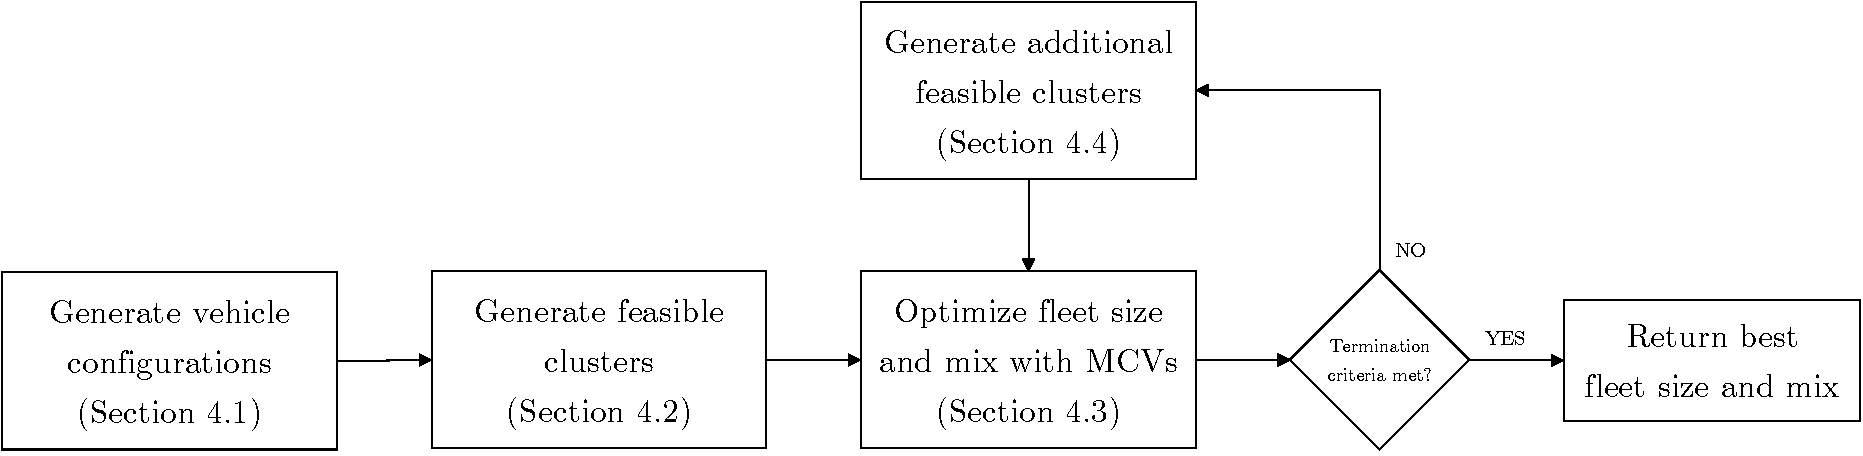
\includegraphics[width=1.0\textwidth]{Imagens/methodology_iterative.pdf}
    \vspace{2.5mm}
    \caption{High-level overview of the matheuristic approach.}
    \label{fig:methodology}
\end{figure}

\subsection{Generate Vehicle Configurations} \label{sec:generate_configurations}

We define the set of vehicle configurations, $V$, based on the available vehicle types and compartments. Specifically, for each vehicle type, we define $2^{|M|}-1$ configurations, where $M$ denotes the set of compartments. For example, the food distributor that inspired this research divides their vehicles into three compartments dedicated to dry ($m^\text{dry}$), refrigerated ($m^\text{ref}$), and frozen ($m^\text{fro}$) product types. In this case, we consider the following subsets of $M$, each defining a configuration: $\{m^\text{dry}\}$, $\{m^\text{ref}\}$, $\{m^\text{fro}\}$, $\{m^\text{dry}, m^\text{ref}\}$, $\{m^\text{dry}, m^\text{fro}\}$, $\{m^\text{ref}, m^\text{fro}\}$, and $\{m^\text{dry}, m^\text{ref}, m^\text{fro}\}$. Therefore, we generate $r \cdot (2^{|M|}-1)$ vehicle configurations, with $r$ denoting the number of vehicle types.

Note that our procedure includes generating \acp{SCV} dedicated to a particular product type (namely, the configurations arising from the singletons $\{m^\text{dry}\}$, $\{m^\text{ref}\}$, and $\{m^\text{fro}\}$), enabling our fleet size and mix optimization model to select either \acp{MCV} or \acp{SCV} based on their respective cost structures and characteristics. Since we consider multiple heterogeneous vehicle types, our procedure generalizes the approach presented by \cite{OstermeierHübner2018}, who only consider one vehicle type. Lastly, since we consider \acp{MCV} with flexible compartments, note that our optimization model then defines the specific load capacity associated with each compartment of the selected vehicle configurations.


\subsection{Generate Feasible Customer Clusters}
\label{sec:generate_feasible_clusters}

After defining the set of vehicle configurations, $V$, we generate feasible clusters of customers that can be served by at least one configuration while satisfying maximum load capacity and route duration constraints. Specifically, for each configuration $v \in V$, we apply a variety of clustering techniques to create clusters that are feasible for that configuration. These techniques include $k$-means, $k$-medoids, Gaussian mixture models, and hierarchical (agglomerative) clustering (see \ref{app:data:clustering} for a summary of the clustering techniques). While these are standard clustering techniques, we adapt them to account for both geographical and demand proximity between customers. Furthermore, we apply a split-and-merge procedure to the resulting set of clusters, not only to validate feasibility but also to enrich the final set of clusters that serves as input to our optimization phase.

Note that, as described in Section \ref{sec:problem_definition}, the resulting clusters do not necessarily partition the set of customers, as some customers may appear in more than one cluster. However, the actual allocation of each customer to a given cluster (and, therefore, vehicle configuration) is then determined during our optimization phase (see Section \ref{sec:model_formulation}). 

In the following, we explain how load capacity and route duration feasibility are verified, as well as how the distance metric is adapted for the clustering techniques used.

\subsubsection{Load Capacity and Route Duration Feasibility Checks} \label{sec:feasibility_checks}

To ensure the creation of feasible customer clusters, we perform both capacity and route duration feasibility checks. Capacity constraints require that the total demand across all product types within a cluster does not exceed the total capacity of the corresponding vehicle configuration, while route duration constraints ensure that the total travel time to serve a cluster remains within a prescribed threshold. Since the total capacity required by a cluster can be readily determined by summing the demand across all product types, we now focus on how route durations are computed within the context of our tactical decision-making problem. We then explain how both capacity and route duration feasibility are ensured through a split-and-merge procedure.

\paragraph{Computation of vehicle route durations}

Depending on the application context, our matheuristic allows decision-makers to verify maximum route duration constraints using one of two methods: \ac{CA} or a state-of-the-art routing solver. \ac{CA} is a widely used technique to approximate vehicle routing costs in large-scale integrated decision-making problems where operational routing decisions play a subordinate role, such as location-routing \citep{winkenbach2016, Pina2022}, workforce sizing and routing \citep{mandal2025tactical}, and fleet design and routing problems \citep{franceschetti2017strategic, zinnenlauf_2024}. In this work, we consider the seminal \ac{CA} formula proposed by \cite{beardwood1959shortest}, extended to incorporate vehicle setup times, customer service times, and depot-to-cluster travel times. Specifically, for a given cluster $k \in K_v$ with $n$ customers distributed over a service area $A$, we approximate the total routing time of serving the cluster using vehicle configuration $v \in V$ as
\begin{equation}
    t_{vk} \approx 2 \cdot \delta_{vk} + \beta \cdot \sqrt{n \cdot A} + \gamma \cdot n,
\end{equation}
where $\delta_{vk}$ is the line-haul travel time between the depot and the centroid of the cluster, $\gamma$ the customer service time, and $\beta$ is a non-negative constant. The second term corresponds to the well-known \ac{BHH} approximation presented by \cite{beardwood1959shortest} (see \cite{silva2022demand} for a recent work showing the quality of this approximation to produce near-optimal estimates). 

Note that an alternative method for computing vehicle route durations is to employ an existing routing solver. In our matheuristic implementation (see our GitHub repository), decision-makers can also use the \textsc{PyVRP} library developed by \cite{wouda_pyvrp_2024}, which is recognized as a state-of-the-art vehicle routing solver. While this approach might enhance vehicle routing time estimations, it often requires substantially more computational time than the \ac{CA}-based approach, especially when dealing with large instances.

\begin{algorithm}[H]
\caption{Recursive Cluster Splitting}
\label{alg:recursive_split}
\begin{algorithmic}[1]
\Function{\textproc{SplitCluster}}{Cluster, DepthLevel, MaxDepth}
    \If{\textproc{ExceedsConstraints}(Cluster) \textbf{and} DepthLevel $<$ MaxDepth}
        \State SubClusters $\gets$ \textproc{Split}(Cluster, 2) \Comment{Split cluster into two sub-clusters}
        \For{\textbf{each} SubCluster \textbf{in} SubClusters}
            \State \textproc{SplitCluster}(SubCluster, DepthLevel + 1, MaxDepth)
        \EndFor
    \Else
        \State \textproc{AddValidCluster}(Cluster) %: $K_v = K_v \cup \{k\}$
    \EndIf
\EndFunction
\end{algorithmic}
\end{algorithm}

\paragraph{Split-and-merge procedure}
After computing vehicle route durations, we verify both load capacity and route duration constraints through a split-and-merge procedure. First, we conduct a recursive binary splitting, as detailed in Algorithm \ref{alg:recursive_split}. When cluster $k \in K_v$ exceeds either the total capacity or the maximum route duration limit associated with vehicle configuration $v \in V$ (i.e., when $\sum_{i \in k} \sum_{p \in P} d_{ip} > Q_v$ or $t_{vk} > T_v$, respectively), the cluster is recursively divided into two subclusters. 
This splitting process continues until all resulting clusters satisfy both constraints or a predefined maximum recursion depth is reached.

Since Algorithm \ref{alg:recursive_split} may produce small clusters with only a few customers, we then apply a merging step to all clusters $k \in K$ such that $|k| < \eta$, where $\eta$ denotes a minimum cluster size. For each such small cluster $k_i$, we define a neighborhood consisting of the $
\Delta$ closest clusters regarding centroid-to-centroid distance. Then, for each neighboring cluster $k_j$, we check whether the combined cluster $k_i \cup k_j$ can be feasibly served by a single vehicle configuration, considering both load capacity and route duration constraints. If feasible, we update the set of clusters by adding $k_i \cup k_j$, i.e., $K = K \cup \{k_i \cup k_j\}$. Note that a similar merging procedure is used during our improvement phase, but only to promising clusters selected in optimal solutions (see Section \ref{sec:improvement_phase}).

\subsubsection{Distance Metric} \label{distance_metric}

Lastly, we describe how we modify the distance metric to account for both geographic and demand proximity when generating clusters.
To enhance the clustering process, we create a composite distance metric that combines geographical distance and product demand similarity into a single value. 
We thus define a composite distance function $D_{ij}$ between customers $i, j \in N$ as
\begin{equation}
    D_{ij} = \lambda \cdot D^{\text{geo}}_{ij} + (1-\lambda) \cdot D^{\text{prod}}_{ij}
\end{equation}
where $\lambda \in [0,1]$ establishes the weight between geographical proximity, measured by the geographical distance $D^{\text{geo}}_{ij}$, and product demand similarity, given by the product distance $D^{\text{prod}}_{ij}$ (we refer the reader to \ref{app:data:clustering} for the specific value of $\lambda$ used in each clustering technique considered). Notably, we compute the product distance (measuring demand similarity) as the cosine distance between weighted demand composition profiles, where demands are normalized by total volume and weighted equally across product types. 

\subsection{Optimize Fleet Size and Mix with Heterogeneous \acp{MCV}} \label{sec:model_formulation}

Based on the generated set of clusters, we now define the \ac{MCV} fleet size and mix that minimizes the total costs incurred to meet each individual customer's demand. It is worth recalling that the total cost of serving cluster $k \in K_v$ with vehicle configuration $v \in V$, denoted by $c_{vk}$, includes both a fixed cost (associated with setting up the vehicle’s compartments and dispatching it) and a variable cost that depends on the distance traveled to serve the cluster. Notably, such fixed costs capture the additional operational effort required to set up and operate a \ac{MCV} configuration, as opposed to a \ac{SCV} configuration.

Let $x_{vk}$ be a binary decision variable equal to 1 if and only if vehicle configuration $v \in V$ serves cluster $k \in K_v$. Our integer programming model reads
\newpage
\begin{subequations} \label{P}
\begin{equation}
    \text{minimize} \quad \sum_{v \in V}\sum_{k \in K_v} c_{vk} \cdot x_{vk}, \label{1}
\end{equation}

subject to
\begin{align}
\sum_{k \in K_i} \sum_{v \in V_k} x_{vk} \ & = \ 1, & i \in N, \label{2} \\
\sum_{v \in V_k} x_{vk} \ & \leq \ 1 , &  k \in K, \label{3} \\
x_{vk} \ & \in \  \{0,1\}, & v \in V, k \in K_v. \label{4}
\end{align} 

The objective function \eqref{1} minimizes the total fixed and variable costs.
Constraints \eqref{2} force to serve each individual customer $i \in N$.
Constraints \eqref{3} ensure that each cluster is visited by at most one vehicle configuration. 
Lastly, Constraints \eqref{4} define the domain of the decision variables.

Note that, after solving Problem \eqref{P}, the specific load capacity required for each compartment of the selected vehicle configurations can be readily determined by summing the demand for each product type across all customers in the respective cluster.

\paragraph{Multi-stop delivery policy} Note that Constraints \eqref{2} enforce a \emph{single-stop policy}, where the entire demand for each product type of each customer must be fully served by a single vehicle. Let us introduce the following additional notation to accommodate a multi-stop delivery policy. Let $P_i$ be the set of product types demanded by customer $i \in N$. We define $S_i^p=\{P' \subseteq P_i: p \in P'\}$ as the set of all subsets of $P_i$ that contain product $p \in P_i$. Lastly, for each product type $p \in P_i$, let $K_i^s$ be the subset of clusters containing customer $i \in N$ that can serve the demand of all product types in $s \in S_i^p$. Thus, the following constraints
\begin{equation}
    \sum_{s \in S_i^p} \sum_{k \in K_i^s} \sum_{v \in V_k} x_{vk} \ = \ 1, \qquad i \in N, p \in P_i,
\end{equation}
\end{subequations}
must replace Constraints \eqref{2} in Problem \eqref{P} to allow multiple deliveries per customer.

\subsection{Improvement Phase} \label{sec:improvement_phase}

We perform an improvement phase on the \ac{MCV} fleet size and mix found by Problem \eqref{P}.
Specifically, after solving Problem \eqref{P} for a given set of clusters $K$, we consider each pair of clusters $(k_i, k_j)$ selected in the optimal solution $\boldsymbol{x}^*$ (i.e., $x^*_{k_i,v_i} = 1$ and $x^*_{k_j,v_j} = 1$ for some $v_i, v_j \in V$), check if a single vehicle configuration can feasibly serve them together based on the load capacity and route duration constraints, and, if feasible, update the set of clusters by adding $k_i \cup k_j$, i.e., $K = K \cup \{k_i \cup k_j\}$. After finishing updating the set of clusters, we solve Problem \eqref{P} and repeat this procedure until no further improvement can be reached. Note that, unlike the merging procedure performed during the clustering phase (see Section \ref{sec:generate_feasible_clusters}), which considers only small clusters that are geographically close, our improvement phase evaluates all possible pairs of clusters (selected in the optimal solution at hand) regardless of their size or spatial proximity.

\section{\textsc{FleetMix}: A Spec-Driven Python Package} \label{sec:fleetmix}

\textsc{FleetMix} is the executable companion to our matheuristic: a Python package that implements all algorithms and models presented in Section \ref{sec:solution_approach}. Available on \href{https://pypi.org/project/fleetmix/}{\texttt{PyPI}} and at \url{https://github.com/ekohan/fleetmix} under the MIT license, \textsc{FleetMix} serves two audiences. Researchers can reproduce our results of Section \ref{sec:synthetic_results} with a single command and extend the algorithms by swapping components, and practitioners can deploy our matheuristic directly in production. The version used for this paper (\href{https://github.com/ekohan/fleetmix/releases/tag/v1.0.0}{\texttt{v1.0.0}}) is permanently archived to ensure reproducibility.

\subsection{Architecture and Design}

\textsc{FleetMix} implements our matheuristic through four core modules that mirror the paper's structure: (i) a clustering engine that generates feasible customer clusters using the techniques described in Section \ref{sec:generate_feasible_clusters}, (ii) an optimization core that solves the integer programming formulation presented in Section \ref{sec:model_formulation}, (iii) a post-optimization refinement module implementing the improvement phase detailed in Section \ref{sec:improvement_phase}, and (iv) a benchmarking framework for systematic evaluation.

The implementation uses well-defined interfaces between components. Researchers can substitute alternative clustering algorithms, route time estimators, or \ac{MILP} solvers without modifying other modules. This modularity is systematically documented in our specification system, which serves as the blueprint for the entire architecture.

\subsection{Specification System}

To address the semantic gap between mathematical description and software implementation in computational research, we connect the paper's mathematical formulation to its software through machine-readable specification documents. Each specification details a component's mathematical basis, interface contract, implementation, and usage examples. For example, \href{https://github.com/ekohan/fleetmix/blob/v1.0.0/docs/specs/clustering.md}{\texttt{clustering.md}} documents the split-and-merge procedure (Algorithm \ref{alg:recursive_split}), its default parameters, and how edge cases are handled, providing context that is difficult to extract from source code alone. This specification layer enables reviewers to trace equations to implementations and researchers to extend the methodology with confidence.

Table \ref{tab:spec_traceability} illustrates this traceability, mapping key elements of our matheuristic from the paper to the corresponding software counterparts.

\begin{table}[htbp]
  \centering
  \caption{Traceability between paper sections, specification documents, and implementation modules.}
  \small
  \renewcommand{\arraystretch}{1.2}
  \begin{tabular}{@{}p{0.20\textwidth}p{0.34\textwidth}p{0.36\textwidth}@{}}
    \toprule
    \textbf{Paper Section} & \textbf{Specification Document} & \textbf{Implementation Module} \\
    \midrule
    \S\ref{sec:generate_configurations} Vehicle Configs & \href{https://github.com/ekohan/fleetmix/blob/v1.0.0/docs/specs/vehicle_configurations.md}{\texttt{vehicle\_configurations.md}} & \href{https://github.com/ekohan/fleetmix/blob/v1.0.0/src/fleetmix/utils/vehicle_configurations.py}{\texttt{utils/vehicle\_configurations.py}} \\[2pt]
    \S\ref{sec:generate_feasible_clusters} Clustering & \href{https://github.com/ekohan/fleetmix/blob/v1.0.0/docs/specs/clustering.md}{\texttt{clustering.md}} & \href{https://github.com/ekohan/fleetmix/blob/v1.0.0/src/fleetmix/clustering/generator.py}{\texttt{clustering/generator.py}} \\[2pt]
    \S\ref{sec:model_formulation} Optimization & \href{https://github.com/ekohan/fleetmix/blob/v1.0.0/docs/specs/optimization.md}{\texttt{optimization.md}} & \href{https://github.com/ekohan/fleetmix/blob/v1.0.0/src/fleetmix/optimization/core.py}{\texttt{optimization/core.py}} \\[2pt]
    \S\ref{sec:improvement_phase} Improvement & \href{https://github.com/ekohan/fleetmix/blob/v1.0.0/docs/specs/post_optimization.md}{\texttt{post\_optimization.md}} & \href{https://github.com/ekohan/fleetmix/blob/v1.0.0/src/fleetmix/post_optimization/merge_phase.py}{\texttt{post\_optimization/merge\_phase.py}} \\
    \bottomrule
  \end{tabular}
  \label{tab:spec_traceability}
\end{table}

\subsection{Usage}

\textsc{FleetMix} exposes three interfaces. The command-line tool serves as the primary entry point (e.g., \lstinline|fleetmix optimize --demand customers.csv --config fleet.yaml|), and the command \lstinline|fleetmix reproduce-paper| regenerates every experiment in Sections~\ref{sec:synthetic_results} and~\ref{sec:case_study}. The Python API (\lstinline|import fleetmix as fm|) enables programmatic integration. The web interface allows interactive parameter exploration without coding. All three interfaces use identical input-output schemas, ensuring reproducibility across modalities. The repository includes worked examples: \href{https://github.com/ekohan/fleetmix/blob/v1.0.0/examples/custom_clustering.py}{\texttt{custom\_clustering.py}} implements a round-robin clustering method, \href{https://github.com/ekohan/fleetmix/blob/v1.0.0/examples/custom_route_time.py}{\texttt{custom\_route\_time.py}} provides a straight-line route time estimator, \href{https://github.com/ekohan/fleetmix/blob/v1.0.0/examples/custom_solver_adapter.py}{\texttt{custom\_solver\_adapter.py}} integrates a solver with relaxed optimality gap, and \href{https://github.com/ekohan/fleetmix/blob/v1.0.0/examples/heterogeneous_fleet.py}{\texttt{heterogeneous\_fleet.py}} demonstrates configuring mixed fleets with product-specific vehicle constraints.

\section{Effectiveness of the Matheuristic Approach} \label{sec:synthetic_results}

In this section, we present a detailed computational study to test the effectiveness of our matheuristic. We run all experiments on a standard workstation (Apple Silicon M3, 2024) with 8 CPU cores and 24 GB of RAM. The implementation was developed in Python 3.12, using Gurobi 12.0.2 as a \ac{MILP} solver. Throughout this section, and based on preliminary experiments, we set $\eta = 5$ customers and $\Delta = 50$ to define neighboring clusters when applying our merging procedure described in Section \ref{sec:generate_feasible_clusters}.

\subsection{Test Instances}

As discussed in Section \ref{sec:literature}, our work is the first to address a tactical fleet size and mix problem involving heterogeneous \acp{MCV} with flexible compartments. Therefore, to the best of our knowledge, there are no benchmark instances or solution approaches in the existing literature. To address this limitation, we use the publicly available instances generated by \cite{henke2015multi} and \cite{henke2019branch} for their homogeneous \ac{MCVRP} with flexible compartments, which are one of the works closest to ours. These instances can be categorized as $|N|\_|P|\_|M|\_s$, where $|N|$ denotes the number of customers, $|P|$ the number of product types, $|M|$ the number of compartments, and $s$ a supply parameter (according to \cite{henke2015multi}, e.g., $s=1$ means that each customer demands at least one product type and at most one third of the available product types). We consider instances with three product types, three compartments (i.e., each compartment is dedicated to one product type), and $s \in \{1,2,3\}$. For the instances of \cite{henke2015multi}, this results in a total of 150 instances with 10 customers and three instances with 50 customers. From \cite{henke2019branch}, a total of 45 instances are available, five for each number of customers $|N| \in \{10,15,..., 45, 50\}$.

To evaluate the effectiveness of our matheuristic, we compare our results with those of \cite{henke2015multi} and \cite{henke2019branch}, which are also publicly available in their manuscript. 
However, to ensure a fair comparison, we adopt the following considerations, recognizing that we address a tactical fleet size and mix problem with heterogeneous vehicles rather than an operational routing problem with homogeneous vehicles. 
First, since the cost structure of a fleet size and mix problem is typically driven by fixed vehicle costs, which are not considered by \cite{henke2015multi} and \cite{henke2019branch}, we focus on comparing the number of vehicles to avoid misleading conclusions from incomparable cost structures. Note that the number of vehicles is an input parameter for the \ac{MILP} model and solution approaches proposed by \cite{henke2015multi} and \cite{henke2019branch}, which they computed by solving a bin packing problem when generating their instances.
Second, we only consider homogeneous \acp{MCV} (i.e., a single vehicle type) when generating vehicle configurations (see Section \ref{sec:generate_configurations}).
Third, since \cite{henke2015multi} and \cite{henke2019branch} do not impose route duration constraints, we do not enforce these constraints when generating feasible customer clusters (see Section \ref{sec:generate_feasible_clusters}).
Lastly, in line with \cite{henke2015multi} and \cite{henke2019branch}, we consider a multi-stop delivery policy when solving Problem \eqref{P} (see Section \ref{sec:model_formulation}).

\subsection{Results}

Table \ref{tab:comparison_vehicles} summarizes the comparison between the number of vehicles obtained by our matheuristic and those achieved by \cite{henke2015multi} and \cite{henke2019branch} through their bin packing approach (we refer the reader to our GitHub repository for detailed results). The columns in the table report the total instances per category, the number of instances where our matheuristic achieved the same number of vehicles as \cite{henke2015multi} and \cite{henke2019branch}, the number where our matheuristic found fewer vehicles, and the average run time (in seconds) per instance category. 

\begin{table}[htbp]
  \centering
  \caption{Comparison between the number of vehicles obtained by our matheuristic and those of \cite{henke2015multi} and \cite{henke2019branch}.}
  \scalebox{0.8}{
    \begin{tabular}{ccrrrr}
    \toprule
    Benchmark & Category & \multicolumn{1}{c}{Instances} & \multicolumn{1}{c}{\# Same vehicles} & \multicolumn{1}{c}{\# Fewer vehicles} & \multicolumn{1}{c}{Run time (s)} \\
    \midrule
    \multirow{6}[2]{*}{\cite{henke2015multi}} & 10\_3\_3\_1 & 50    & 24    & 26    & 5.0 \\
          & 10\_3\_3\_2 & 50    & 28    & 22    & 5.0 \\
          & 10\_3\_3\_3 & 50    & 35    & 15    & 5.1 \\
          & 50\_3\_3\_1 & 1     & 1     & 0     & 7.3 \\
          & 50\_3\_3\_2 & 1     & 1     & 0     & 8.1 \\
          & 50\_3\_3\_3 & 1     & 1     & 0     & 8.4 \\
    \midrule
    \multirow{9}[2]{*}{\cite{henke2019branch}} & 10\_3\_3\_3 & 5     & 5     & 0     & 5.2 \\
          & 15\_3\_3\_3 & 5     & 5     & 0     & 5.3 \\
          & 20\_3\_3\_3 & 5     & 5     & 0     & 5.3 \\
          & 25\_3\_3\_3 & 5     & 5     & 0     & 5.5 \\
          & 30\_3\_3\_3 & 5     & 5     & 0     & 5.4 \\
          & 35\_3\_3\_3 & 5     & 5     & 0     & 5.7 \\
          & 40\_3\_3\_3 & 5     & 5     & 0     & 5.8 \\
          & 45\_3\_3\_3 & 5     & 5     & 0     & 5.8 \\
          & 50\_3\_3\_3 & 5     & 5     & 0     & 6.5 \\
    \bottomrule
    \end{tabular}%
    }
  \label{tab:comparison_vehicles}%
\end{table}%

Table \ref{tab:comparison_vehicles} shows the effectiveness of our matheuristic in reducing or maintaining the number of vehicles needed compared to the number of vehicles found by \cite{henke2015multi}. For instances with 10 customers, our matheuristic finds solutions with exactly one fewer vehicle in 52\%, 44\%, and 30\% of the instances with supply parameters $s$ equals to 1, 2, and 3, respectively. For larger instances with 50 customers, our matheuristic finds the same number of vehicles as \cite{henke2015multi}.
When compared with \cite{henke2019branch}, Table \ref{tab:comparison_vehicles} reports that our matheuristic consistently finds the same number of vehicles, regardless of the problem size.
Note that, regardless of the instance category, our matheuristic (from generating vehicle configurations to returning the best solution found; see Figure \ref{fig:methodology}) takes less than nine seconds on average.

In summary, these results validate the effectiveness of our matheuristic in finding high-quality solutions while maintaining short computational times.

\section{Real-World Case Study} \label{sec:case_study}

After showing the computational performance of our matheuristic approach, we now present and discuss results from a real-world case study based on the current operations of our industry partner, a leading food distributor based in Bogotá, Colombia. We begin this section by describing our real-world problem instances. We then present and discuss managerial insights regarding the benefits of adopting \acp{MCV}. Lastly, we analyze the resulting fleet composition under different cost structures. 

Throughout this section, we employ the same parameters and computational environment described in Section \ref{sec:synthetic_results}. For transparency, detailed computational results (including run times, which are under 1 minute across all instances and parameter combinations tested) are publicly available at \url{https://github.com/ekohan/fleetmix}.

\subsection{Real-World Problem Instances} \label{sec:real_world_instances}

Our industry partner provided us with a rich dataset containing 70 days of real-world demand information. Each day (i.e., problem instance) provides detailed information about customer locations and the quantities of products requested by product type (frozen, chilled, and dry). Over the 70 days, the number of customers served by the company ranges from 208 to 691, with an average of 379 customers. Below, we explain the main characteristics of the service area and vehicle fleet, as well as the parameter values used.

\paragraph{Service area} 
The service area is located in Bogotá, Colombia, the country's most populous city. Geographically, the service area spans around 1,226 km$^2$. The company serves an average of 379 customers per day from a single depot located on the outskirts of the city. Figure \ref{fig:CaseStudyArea} shows the spatial distribution of customers for a representative day (to protect confidentiality, the node locations have been slightly perturbed).

\begin{figure}[H]
    \centering
    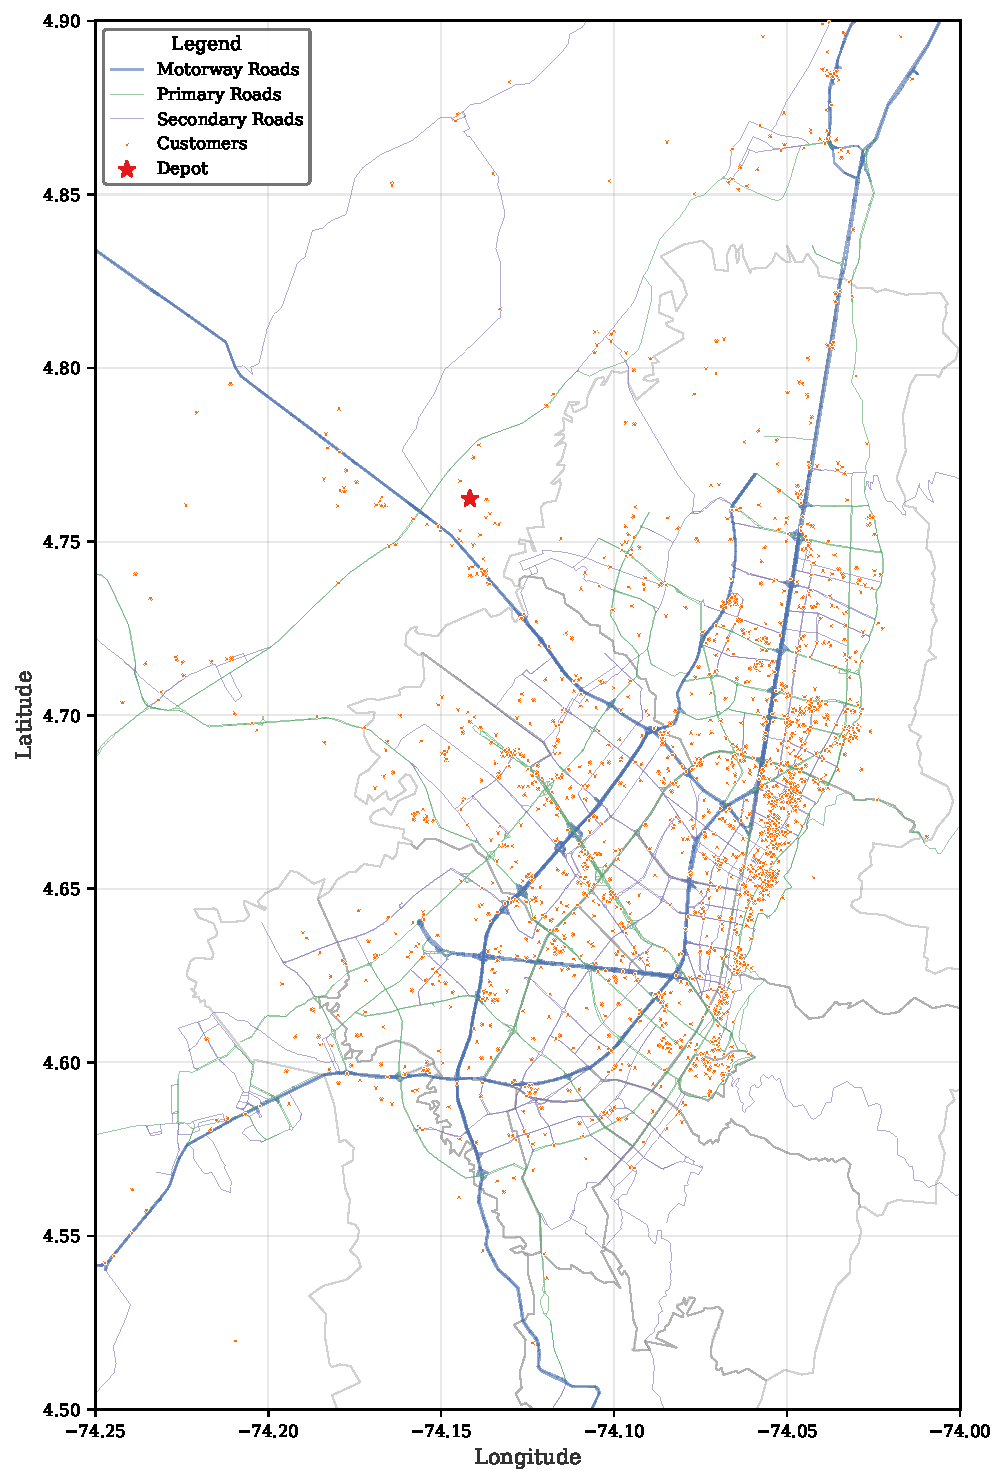
\includegraphics[width=0.7\textwidth]{Imagens/service_area.pdf}
    \caption{Service area and customer distribution.}
    \label{fig:CaseStudyArea}
\end{figure}

\paragraph{Heterogeneous \acp{MCV}}
The company operates a fleet of heterogeneous \acp{MCV}, comprising three vehicle types with flexible compartments.
Before the delivery horizon begins, the company decides the number of each vehicle type to deploy and their respective compartment configurations.
Vehicle Type A has a total capacity of 700 kg and a fixed cost of 80 units; Vehicle Type B has a capacity of 1,300 kg and a fixed cost of 140 units; and Vehicle Type C provides 2,500 kg at a fixed cost of 180 units (costs have been scaled for confidentiality).
Each vehicle type allows seven compartment configurations (see Section \ref{sec:generate_configurations}), with a (homogeneous) setup cost of 10 units per associated compartment. 
Thus, for example, the total fixed cost of using one vehicle of Type C equipped with two compartments (e.g., dry and frozen) is 200 units (i.e., $180 + 2\cdot10$).
We assume that vehicles travel the Euclidean distance between nodes at a constant speed of 30 km/h. Based on the company's recommendation, we set a service time of 25 minutes per stop, which is the average time the company currently takes to deliver food products to their customers (e.g., local restaurants or hotels). The variable vehicle cost is 10 units per operating hour, with a maximum route duration of 10 hours. Lastly, given that our instances involve hundreds of customers (from 208 to 691 customers), we check route duration feasibility through \ac{CA} when generating customer clusters, using a \ac{BHH} constant of $\beta = 0.765$ (see Section \ref{sec:feasibility_checks} and \cite{carlsson2025new} for a detailed discussion of this parameter). 

\subsection{Benefits of Using Multi-Compartment Vehicles}

To understand the benefits of using \ac{MCV} fleets over traditional \ac{SCV} fleets, we assess the effects of varying three key operational parameters: total vehicle capacity, customer service time, and the maximum allowed route duration. We establish the baseline scenario with the parameter values detailed in Section \ref{sec:real_world_instances}, which capture the company’s current operations. For each parameter variation, we compute the impact on fleet size (i.e., the total number of vehicles employed) and total cost (comprising fixed and variable costs associated with using the selected vehicle configurations).

Figure \ref{fig:mean_fleet_and_cost_reduction} illustrates how the average fleet size and total cost change when varying a single parameter by –50\%, –20\%, +20\%, and +50\% relative to the baseline scenario. Results consistently show that adopting \acp{MCV} leads to reductions in both metrics across all parameter combinations. Notably, in the baseline scenario (indicated by the vertical line at 0\% on the horizontal axis of each subplot), using \acp{MCV} reduces the average fleet size by 9.0 vehicles and the average total cost by 18.5\%. To facilitate the interpretation of these results, Table \ref{tab:sensitivity_analysis} reports additional operational metrics: vehicle load utilization (i.e., the average percentage of total vehicle capacity used), the average number of customers served per vehicle, the average route duration (including travel and service times), and the fleet composition (in terms of vehicle types used). We now examine the main direct effects of each parameter variation.

\begin{figure}[htbp]
    \centering
    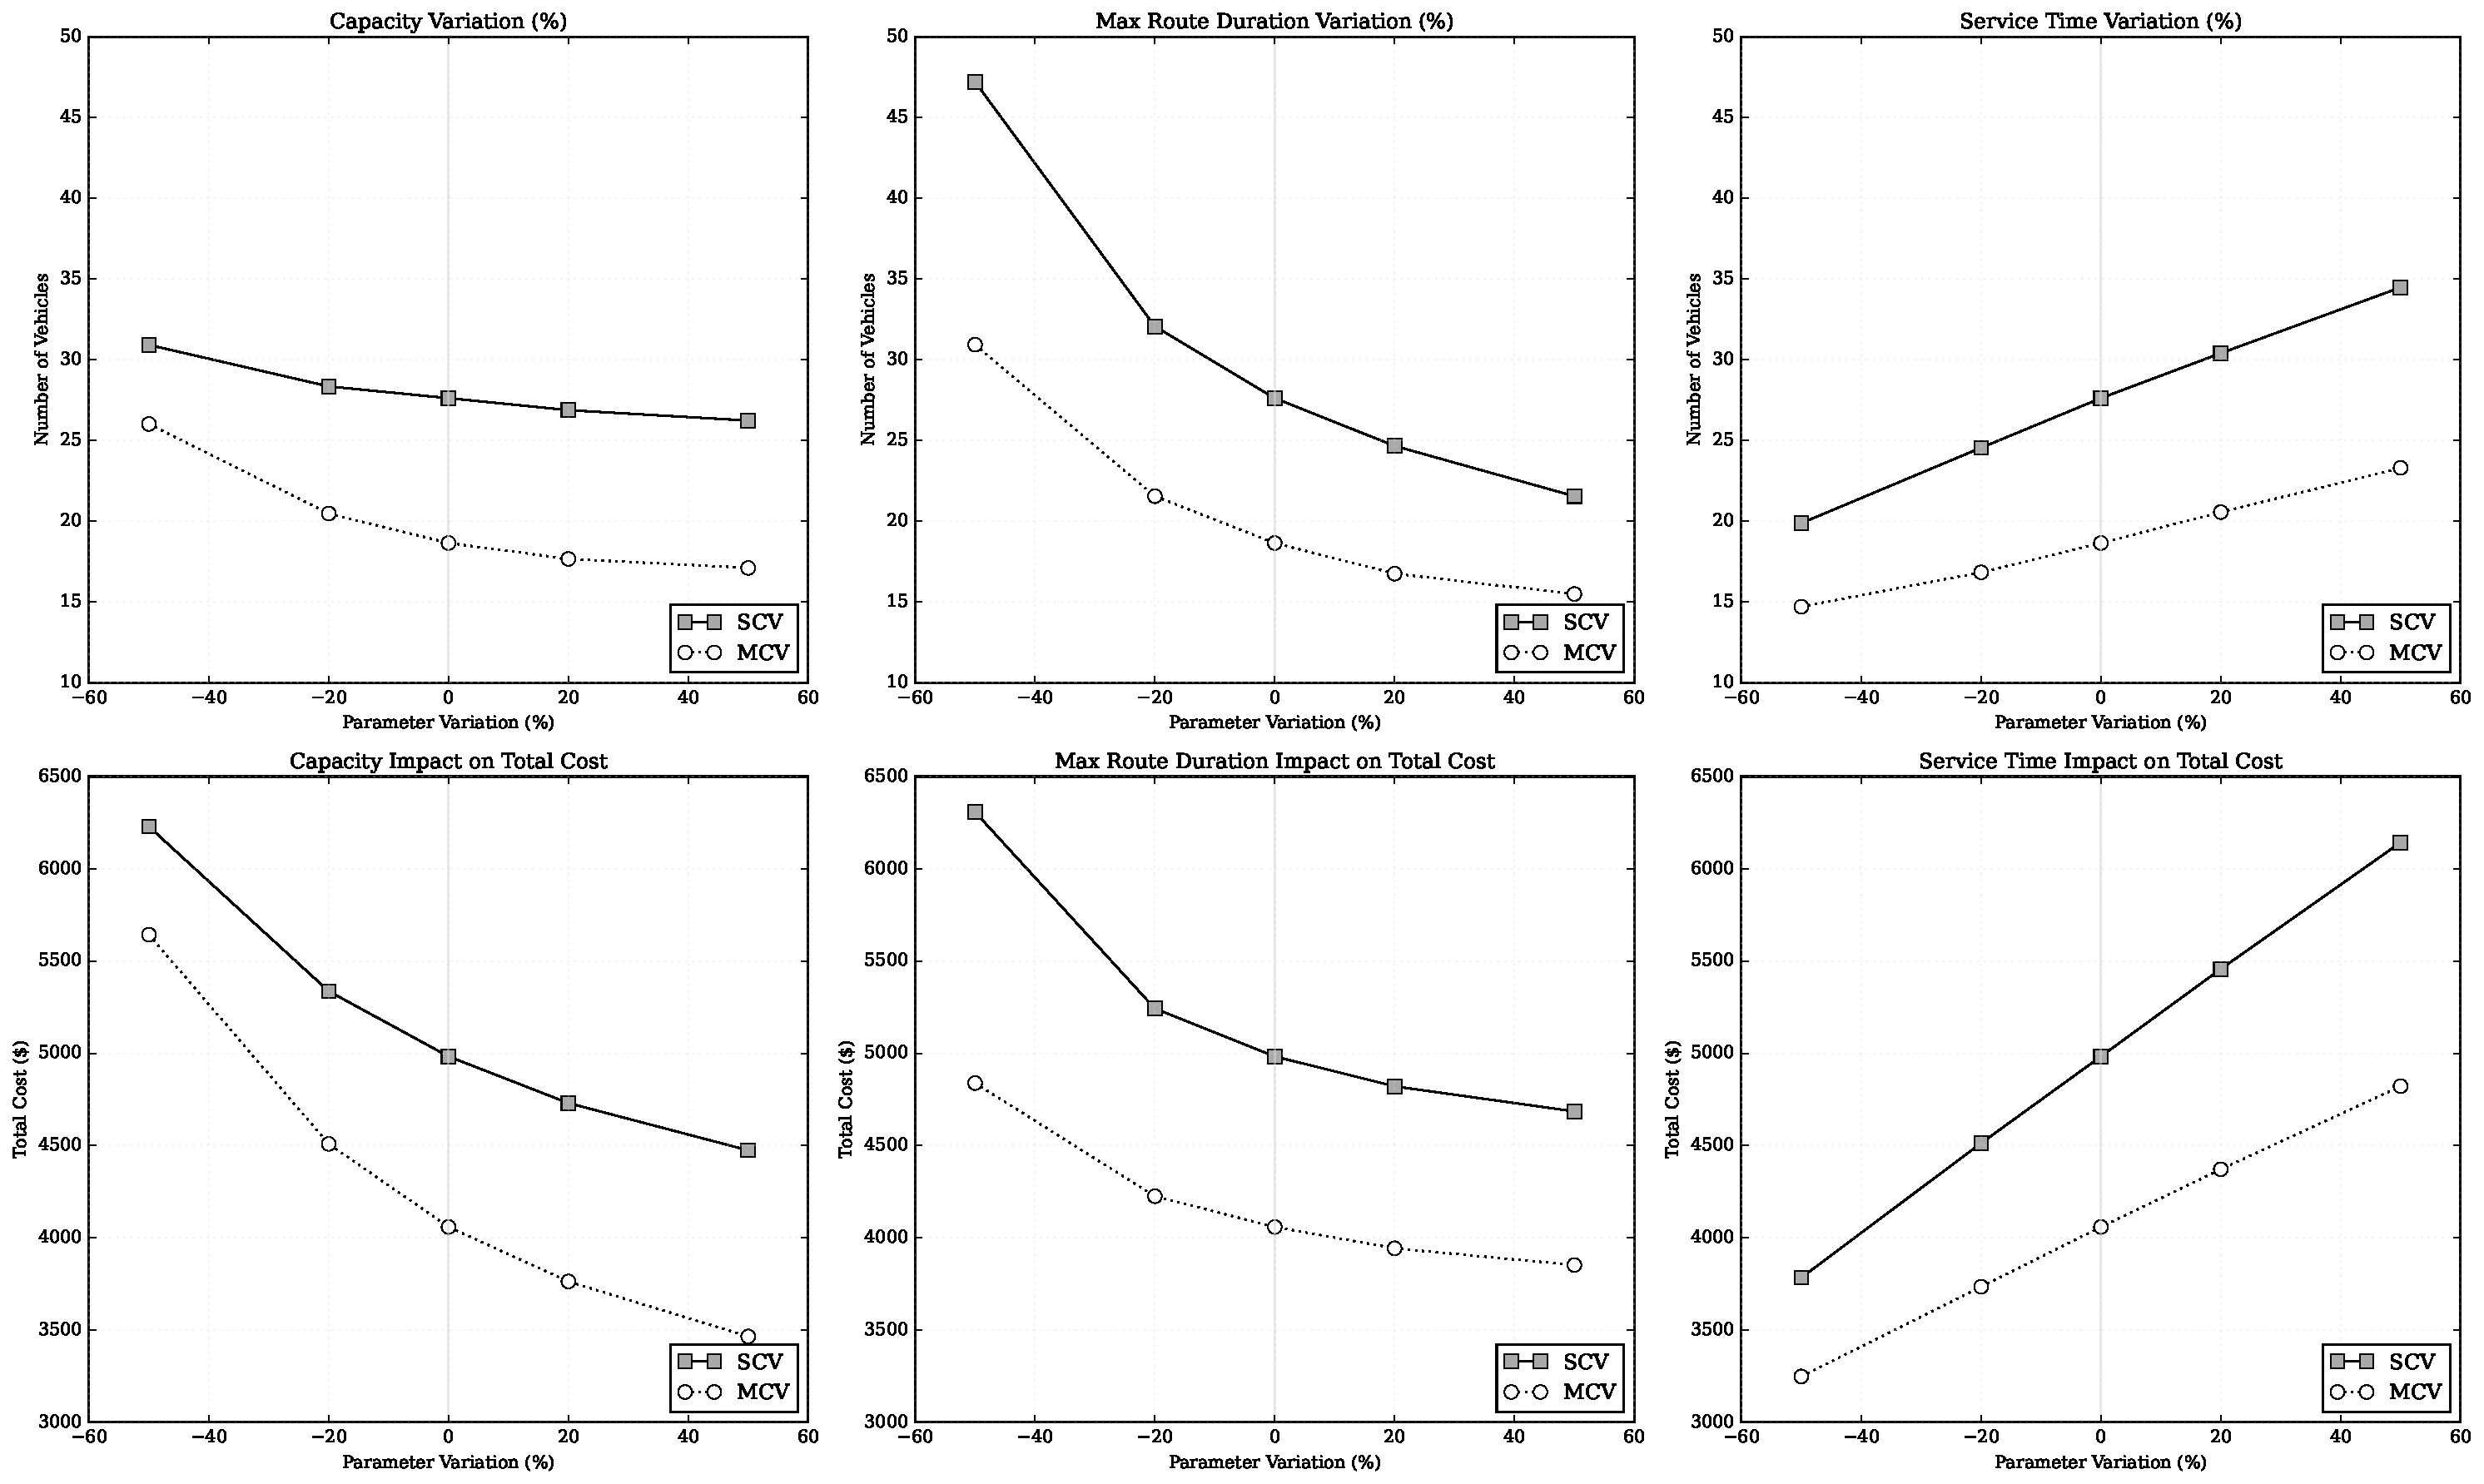
\includegraphics[width=1.0\linewidth]{Imagens/MCV_savings.pdf}
    \vspace{0.1mm}
    \caption{Average fleet size and total cost (over 70 instances) achieved by the \ac{MCV} and \ac{SCV} fleet for each parameter combination.}
    \label{fig:mean_fleet_and_cost_reduction}
\end{figure}

\begin{table}[htbp]
  \centering
  \caption{Average operational metrics (over 70 instances) per parameter variation.}
    \resizebox{\textwidth}{!}{
    \begin{tabular}{lrrrrcrrrrrrrrr}
    \toprule
    \multirow{2}[4]{*}{Parameter} & \multicolumn{1}{c}{\multirow{2}[4]{*}{Variation}} &       & \multicolumn{2}{c}{{\thead{Vehicle load \\ utilization}}} &       & \multicolumn{2}{c}{{\thead{Customers \\ per vehicle}}} &       & \multicolumn{2}{c}{{\thead{Route \\ duration}}} &       & \multicolumn{3}{c}{{\thead{MCV fleet composition}}} \\
\cmidrule{4-5}\cmidrule{7-8}\cmidrule{10-11}\cmidrule{13-15}          &       &       & \multicolumn{1}{c}{MCV} & \multicolumn{1}{c}{SCV} &       & \multicolumn{1}{c}{MCV} & \multicolumn{1}{c}{SCV} &       & \multicolumn{1}{c}{MCV} & \multicolumn{1}{c}{SCV} &       & \multicolumn{1}{c}{Type A} & \multicolumn{1}{c}{Type B} & \multicolumn{1}{c}{Type C} \\
    \midrule
    \multirow{5}[2]{*}{Load Capacity} & -50\% &       & 87.5\% & 85.8\% &       & 10.1  & 12.2  &       & 5.3   & 6.6   &       & 6.2   & 3.0   & 16.9 \\
          & -20\% &       & 86.5\% & 79.6\% &       & 12.4  & 13.4  &       & 6.5   & 7.1   &       & 6.8   & 3.2   & 10.5 \\
          & 0\%   &       & 86.4\% & 75.7\% &       & 13.4  & 13.7  &       & 7.0   & 7.3   &       & 7.5   & 3.7   & 7.5 \\
          & 20\%  &       & 83.6\% & 71.8\% &       & 14.2  & 14.1  &       & 7.4   & 7.5   &       & 8.8   & 3.0   & 5.8 \\
          & 50\%  &       & 81.7\% & 66.4\% &       & 14.6  & 14.4  &       & 7.6   & 7.6   &       & 10.9  & 2.6   & 3.7 \\
    \midrule
    \multirow{5}[2]{*}{Max. Route Duration } & -50\% &       & 77.6\% & 57.1\% &       & 8.1   & 8.0   &       & 4.4   & 4.4   &       & 24.3  & 2.4   & 4.3 \\
          & -20\% &       & 84.9\% & 72.2\% &       & 11.6  & 11.8  &       & 6.1   & 6.3   &       & 11.7  & 3.2   & 6.6 \\
          & 0\%   &       & 86.4\% & 75.7\% &       & 13.4  & 13.7  &       & 7.0   & 7.3   &       & 7.5   & 3.7   & 7.5 \\
          & 20\%  &       & 86.4\% & 78.3\% &       & 15.1  & 15.3  &       & 7.8   & 8.1   &       & 5.2   & 3.2   & 8.4 \\
          & 50\%  &       & 85.6\% & 79.0\% &       & 16.3  & 17.6  &       & 8.5   & 9.3   &       & 3.9   & 2.3   & 9.3 \\
    \midrule 
    \multirow{5}[2]{*}{Service Time} & -50\% &       & 85.6\% & 78.5\% &       & 17.3  & 19.2  &       & 5.2   & 5.9   &       & 3.0   & 2.1   & 9.6 \\
          & -20\% &       & 86.0\% & 77.0\% &       & 15.0  & 15.4  &       & 6.5   & 6.9   &       & 5.4   & 2.9   & 8.5 \\
          & 0\%   &       & 86.4\% & 75.7\% &       & 13.4  & 13.7  &       & 7.0   & 7.3   &       & 7.5   & 3.7   & 7.5 \\
          & 20\%  &       & 85.7\% & 73.6\% &       & 12.2  & 12.4  &       & 7.4   & 7.7   &       & 10.4  & 3.3   & 6.9 \\
          & 50\%  &       & 84.9\% & 70.3\% &       & 10.7  & 11.0  &       & 7.8   & 8.1   &       & 14.4  & 2.8   & 6.1 \\
    \bottomrule
    \end{tabular}%
    }
  \label{tab:sensitivity_analysis}%
\end{table}%

\paragraph{Effects of vehicle capacity} 
Figure \ref{fig:mean_fleet_and_cost_reduction} shows that vehicle capacity has only a modest effect on fleet size for both \ac{MCV} and \ac{SCV} cases. For instance, a 50\% reduction in the total vehicle capacity results in only a slight increase in the number of vehicles (approximately from 18.7 to 26.0 for \acp{MCV} and from 27.6 to 30.9 for \acp{SCV}) yet leads to a sharp rise in total cost. 
Table \ref{tab:sensitivity_analysis} supports these findings: when load capacity is reduced by 50\%, the \ac{MCV} fleet composition shifts toward a much higher share of large, more expensive Type C vehicles (from 7.5 to 16.9 vehicles on average), while the number of small, less expensive Type A vehicles decreases. 
This substitution keeps the total number of vehicles required almost unchanged because larger vehicles can absorb the reduced capacity, but it substantially increases total costs.
These results show that changes in capacity mainly affect total cost rather than fleet size, since the fleet composition can be adjusted without substantially changing the number of vehicles required.

\paragraph{Effects of maximum route duration} 
As shown in Figure \ref{fig:mean_fleet_and_cost_reduction}, the response to changes in maximum route duration is highly asymmetric. For instance, when the maximum route duration is reduced by 50\%, the number of vehicles increases by approximately 66\% and 71\% in \ac{MCV} and \ac{SCV} cases, respectively, resulting in a substantial increase in total cost: 19\% for \acp{MCV} and 27\% for \acp{SCV}. Conversely, extending the maximum route duration by 50\% (corresponding to 15 working hours, which exceeds practical operational limits but is included here for illustrative purposes) yields only moderate efficiency gains: the average fleet size decreases by 17\% and 22\% for the \ac{MCV} and \ac{SCV} cases, respectively, with total cost reductions of only 5.1\% and 6.0\%.
This asymmetric response is mainly driven by \ac{MCV} fleet composition: with a 50\% reduction in maximum route duration, small vehicles (Type A) rise quickly from 7.5 to 24.3, since limited time on route prevents efficient use of (more expensive) larger vehicles. In contrast, when duration is extended by 50\%, the share of large vehicles (Type C) increases from 7.5 to 9.3, but their higher capacity does not translate into a substantial reduction in total fleet size compared to the baseline scenario (e.g., when using \acp{MCV}, the total fleet size is reduced from 18.7 to 15.5 vehicles).
Overall, the results suggest that the company should not focus on extending maximum route durations (i.e., drivers’ working hours) to improve performance, as this provides only limited benefits.

\paragraph{Effects of service time} Figure \ref{fig:mean_fleet_and_cost_reduction} shows that customer service time exhibits the most linear relationship among the parameters studied. If the company manages to reduce service time by 50\% (e.g., through better coordination with customers regarding product unloading and delivery), the average number of \acp{MCV} can be reduced by 3.9 vehicles, while achieving a reduction of 7.7 vehicles when employing a traditional \ac{SCV} fleet.
This pattern is also reflected in Table \ref{tab:sensitivity_analysis}. As service time decreases, vehicles can serve more customers per vehicle in a nearly proportional way (from 13.4 to 17.3 customers for \acp{MCV} and from 13.7 to 19.2 for \acp{SCV} under a 50\% reduction). Similarly, the effective route duration follows the same trend, decreasing almost linearly as service time is reduced (from 7.0 to 5.2 hours for \acp{MCV} and from 7.3 to 5.9 for \acp{SCV}). Because both customers-per-vehicle and route duration scale almost directly with the service time parameter, the total number of required vehicles decreases at a nearly constant rate as service time reduces.
Therefore, this nearly linear relationship means that any effort to reduce service time results in a proportional reduction in both fleet size and total costs.

\subsection{Impact of Cost Structure on Fleet Composition}

Due to the practical challenges associated with managing multiple vehicle types, our industry partner is currently considering the use of a homogeneous vehicle fleet (composed of a single vehicle type). Accordingly, in this section, we examine how the cost structure associated with using \acp{MCV} influences fleet composition decisions. For this analysis, we consider that the vehicles in the fleet have a total load capacity of 2,700 kg and can be designated either as \acp{SCV} or \acp{MCV} with flexible compartment sizes.

For this analysis, we establish a baseline fixed cost of $100$ units for using one \ac{SCV}. The fixed cost for using one \ac{MCV} with configuration $v \in V$ is set as $100 \cdot \left( \alpha + c \cdot (|M_v| - 1) \right)$, where $\alpha \in [1, 2]$ represents the premium factor associated with using \acp{MCV}; $M_v$, with $\emptyset \neq M_v \subseteq M$, is the subset of compartments of vehicle configuration $v \in V$; and $c \in [0, 0.5]$ denotes a fraction of the \ac{SCV} fixed costs incurred per additional compartment. For example, when $\alpha = 1.5$ and $c = 0.2$, the total fixed cost of using one \ac{MCV} with three compartments is $190 = 100 \cdot (1.5 + 0.2 \cdot (3 - 1))$, as there are two additional compartments. All other operational parameter values (e.g., customer service time, variable costs) remain the same as defined in Section \ref{sec:real_world_instances}.

Figure \ref{fig:heatmap} presents the combined effect of the premium factor ($\alpha$) and compartment setup factor ($c$) on fleet composition. The horizontal axis represents the compartment setup factor, which increases from 0\% to 50\% in increments of 10\%. The vertical axis corresponds to the $\alpha$ multiplier, which scales the fixed cost of using one \ac{MCV} from 1.0 to 2.0 in increments of 0.1. Each cell in Figure \ref{fig:heatmap} displays three values: the average \ac{MCV} share in percentage, the number of days (out of 70) in which at least one \ac{MCV} is used, and the number of days in which all vehicles in the fleet are \acp{MCV}, marked with a star.

 \begin{figure}[H]
    \centering
    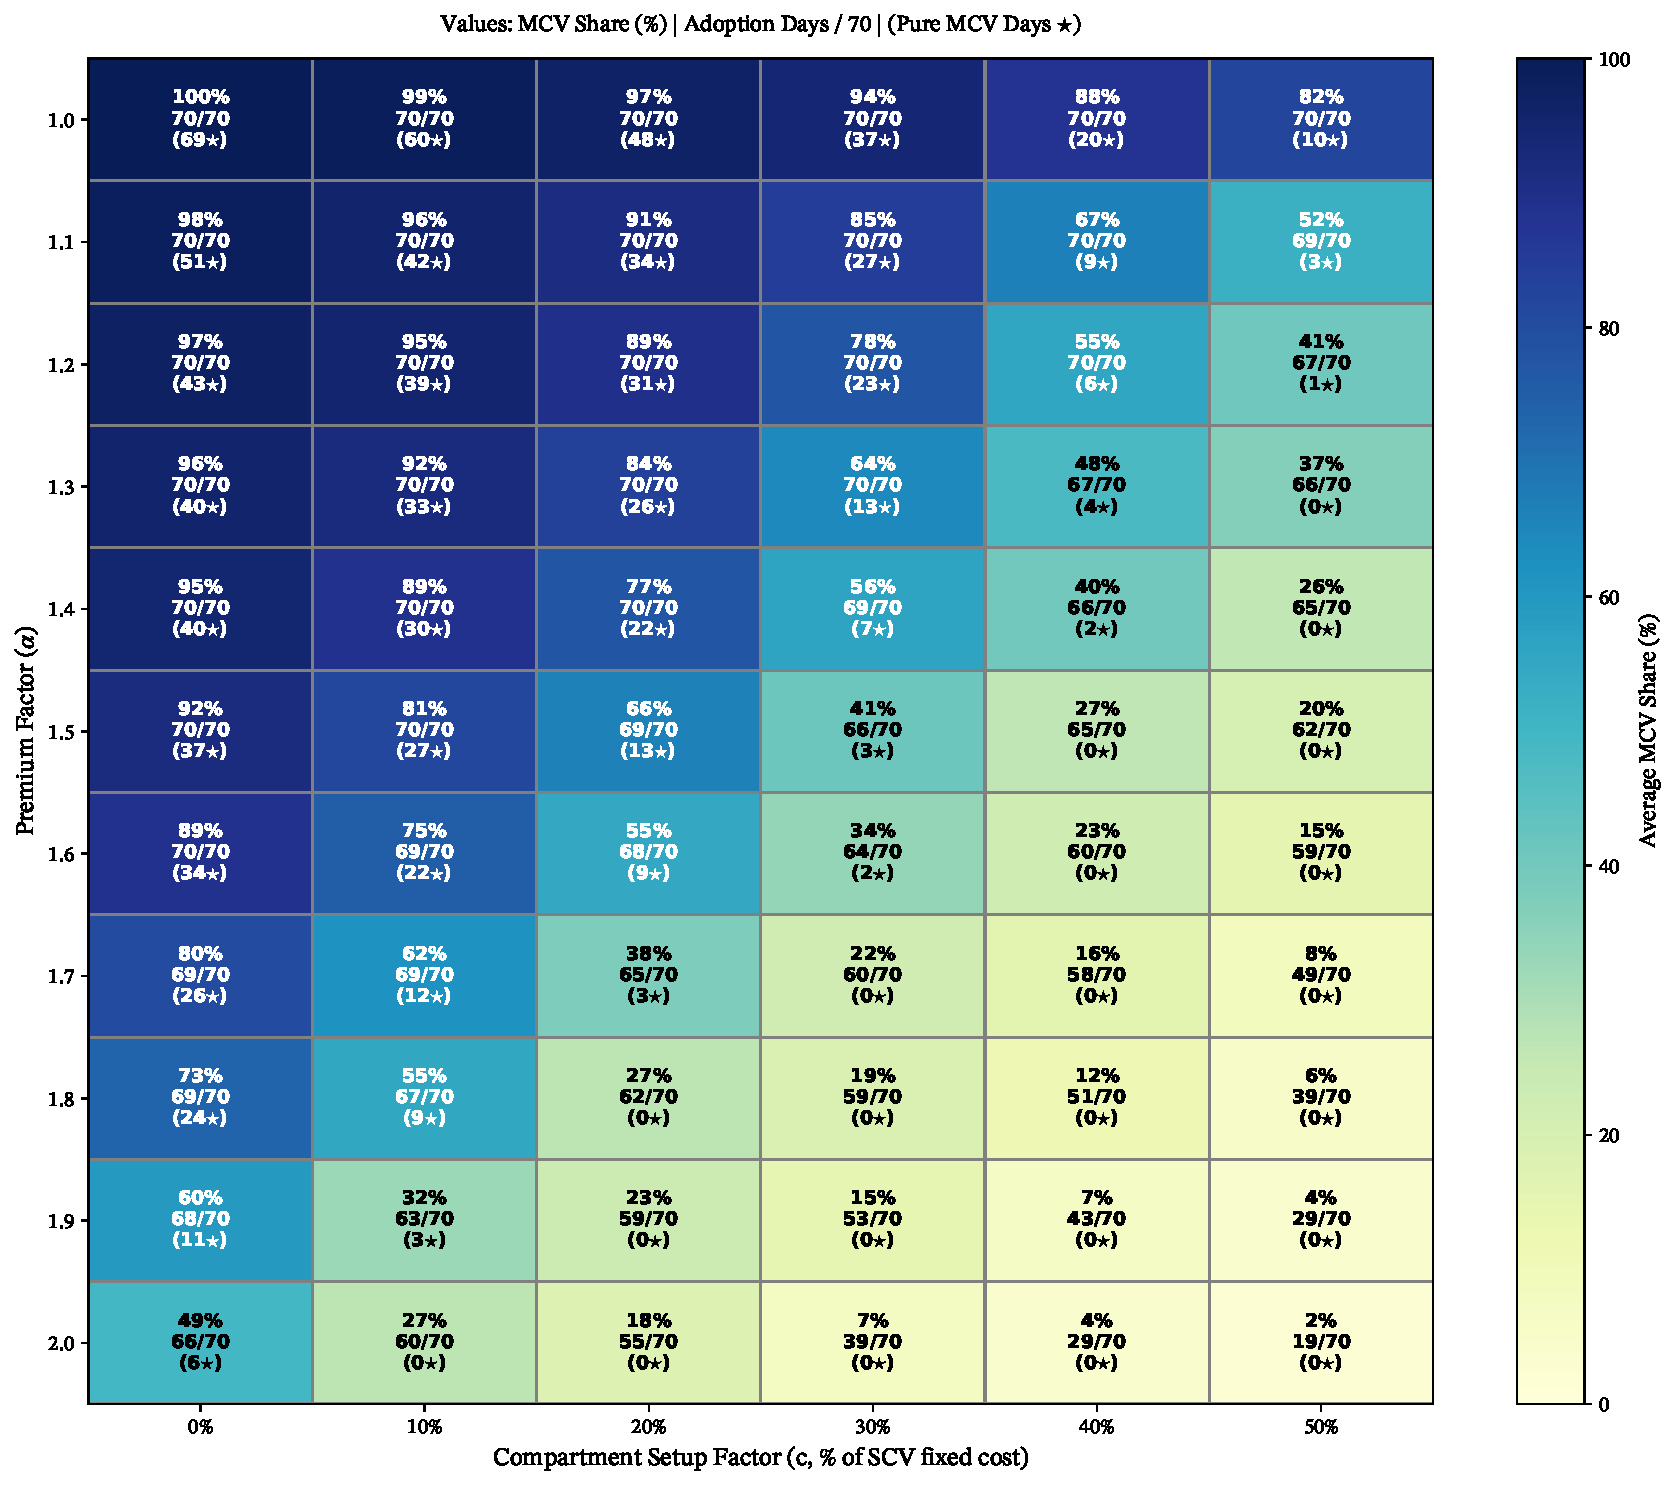
\includegraphics[width=0.95\linewidth]{Imagens/heatmap_mcv_adoption_landscape.pdf}
    \vspace{0.4mm}
    \caption{Effect of premium factor ($\alpha$) and compartment setup factor ($c$) on fleet composition.}
    \label{fig:heatmap}
\end{figure}

Figure \ref{fig:heatmap} shows a clear nonlinear decline in \ac{MCV} adoption as both cost factors increase. When \acp{MCV} are relatively inexpensive compared to \acp{SCV} (e.g., when $\alpha \leq 1.4$ and $c \leq 0.1$, or $\alpha \leq 1.2$ and $c \leq 0.2$), their share consistently represents 90\% or more, indicating that \acp{MCV} dominate the fleet composition and achieve full adoption across all days. However, even modest increases in either parameter rapidly reduce their utilization. When $\alpha \geq 1.5$ and $c \geq 0.3$, the average share of \acp{MCV} falls below 50\%, suggesting that their fixed cost quickly outweighs the operational flexibility offered by compartmentalization. Overall, Figure \ref{fig:heatmap} shows that \ac{MCV} adoption is highly sensitive to the underlying cost structure, indicating that only specific cost parameters make \acp{MCV} an operationally dominant option for fleet composition.

Lastly, Table \ref{tab:fleet_composition_deep_dive} provides a detailed view of how the \ac{MCV} share varies across different compartment setup cost factors, with the premium factor set to $\alpha = 1.6$. As the compartment setup factor increases from $c = 0$ to $c = 0.5$ (i.e., the cost of setting up an additional compartment in a \ac{MCV} represents 50\% of the cost of using a \ac{SCV}), the average \ac{MCV} share rapidly falls from 89\% to 15\%. Initially, this reduction in \ac{MCV} usage might suggest a decrease in total costs, yet the opposite effect occurs. \ac{SCV} fleets require more vehicles to handle incompatible product types separately, leading to an increase in the total fleet size. Consequently, customers are served by multiple vehicles more often. This increase in fleet size raises the total cost by approximately 15\% (from 3,901 to 4,498 cost units), as shown in Table \ref{tab:fleet_composition_deep_dive}.
In summary, these results confirm that compartment setup costs have a strong effect on the daily fleet composition, consistent with the overall pattern observed in Figure \ref{fig:heatmap}.

\begin{table}[htbp]
  \centering
  \caption{Impacts of cost structure when $\alpha = 1.6$. Results averaged over 70 instances.}
  \scalebox{1.0}{
    \begin{tabular}{crrrr}
    \toprule
    \thead{Compartment \\ setup factor ($c$)}   & \multicolumn{1}{c}{\thead{MCV share}} & \multicolumn{1}{l}{\thead{Total cost}} & \multicolumn{1}{c}{\thead{Fleet size}} & \multicolumn{1}{c}{\thead{Visits per \\ customer}} \\
    \midrule
    0.0   & 89\%  & 3,901 & 16.9  & 1.1 \\
    0.2   & 55\%  & 4,292 & 19.0  & 1.3 \\
    0.5   & 15\%  & 4,498 & 23.0  & 1.5 \\
    \bottomrule
    \end{tabular}%
    }
  \label{tab:fleet_composition_deep_dive}%
\end{table}%

\subsection{Managerial Insights} \label{sec:discussion}

The results of our real-world case study provide valuable insights for food distributors and fleet managers considering the adoption of \acp{MCV}. Below, we summarize the key managerial implications derived from our analysis.

\paragraph{Multi-compartment vehicles reduce both total costs and fleet size}
Our results show that adopting \acp{MCV} can lead to substantial performance gains compared with traditional last-mile fleets based on \acp{SCV}. Under the current operating conditions of our industry partner (i.e., our baseline scenario), we find that total costs decrease by 18.5\% and that the total number of required vehicles decreases by an average of 9.0. This improvement comes from the ability of \acp{MCV} to consolidate incompatible product types, allowing vehicles to depart with fuller loads, make fewer stops, and spend less time distributing.

\paragraph{Prioritize reducing service time to boost performance}
Our sensitivity analysis shows that service time is the most practical and effective lever for improving performance, since even small reductions produce clear gains in fleet size and total cost. In contrast, increasing vehicle capacity or extending working hours (i.e., maximum route duration limits) requires additional investment and offers only limited benefits. Changes in capacity have minimal impact on the number of vehicles required, and longer route durations yield only modest improvements. Because shorter customer service times translate almost directly into operational efficiencies, efforts should focus on streamlining delivery and unloading processes (e.g., by improving coordination with customers) rather than investing in larger vehicles or extending working hours.

\paragraph{Deploy multi-compartment vehicles when cost structure supports their flexibility}
Our findings show that fleet size and mix decisions with \acp{MCV} are sensitive to their underlying cost structure. \acp{MCV} are only an operationally dominant option when their fixed-cost structure stays within a favorable range; once premiums or compartment setup costs increase, the fleet composition shifts toward \acp{SCV}. This shift forces more vehicles onto the road and increases how often customers are visited by multiple vehicles, thereby increasing total costs.

\section{Conclusions} \label{sec:conclusions}

\acfp{MCV} are among the most effective vehicle technologies that food distributors can employ to consolidate deliveries of multiple product types while maintaining their specific temperature and loading conditions. Motivated by our collaboration with a major food distributor operating in Bogotá, Colombia, we investigate the design of last-mile delivery fleets involving heterogeneous \acp{MCV} with flexible compartment sizes. Specifically, the decision-making problem faced by the company considers three interconnected decisions: (i) the number of each vehicle type to use, (ii) the type and size of each compartment assigned to each vehicle, and (iii) the distribution plan for each vehicle. The objective is to minimize total logistics costs, which comprise both fixed and variable costs associated with selecting and utilizing vehicles.

To solve this problem, we propose a novel matheuristic approach based on a cluster-first, fleet design-second scheme. Our matheuristic can accommodate several real-world characteristics of modern food distribution operations, including homogeneous and heterogeneous vehicles with fixed or flexible compartment sizes; a comprehensive cost structure that allows including fixed costs, compartment-dependent costs, and variable (distance or time-dependent) costs; and single- and multiple-stop delivery policies. To facilitate the application of our matheuristic, we create \textsc{FleetMix}, an open-source Python package (MIT license, PyPI). Its implementation follows specifications linking the paper's methodology to its software realization, uses defined interfaces to allow for systematic adaptation of its components, and includes a benchmarking tool to ensure verifiable replication of our results.

Using established synthetic instances from the literature, we show that \textsc{FleetMix} achieves high-quality fleet designs compared to existing solution approaches. Through a real-world case study informed by real data from our partner industry company, we derive several managerial insights into the value of using \acp{MCV}. Our results show that, due to their ability to consolidate multiple product types, \acp{MCV} can substantially reduce total logistics costs and fleet size by enabling vehicles to depart with fuller loads and perform more efficient routes. We also find that reducing customer service time is the most effective lever for improving performance compared with increasing vehicle capacity or extending operating hours.

Since our work is among the first to address the tactical design of last-mile delivery fleets with \acp{MCV}, there are several opportunities for future work. 
First, while this is a challenging optimization problem, future research could focus on developing exact solution approaches that can solve practical problem instances to proven optimality. Here, one could develop a column generation-based scheme and use our set partitioning formulation presented in Section \ref{sec:solution_approach}.
Second, future work can also extend \textsc{FleetMix} to accommodate other real-world characteristics, such as other cost components (e.g., loading and unloading costs, as in \cite{hubner2019multi}) and time windows.
Lastly, a stochastic version of the problem, where tactical fleet size and mix decisions are made before customer demand is known, will be a challenge to address.

\newpage
\bibliographystyle{apalike}
\biboptions{authoryear}
\bibliography{mybib.bib}

\newpage
\begin{appendix}
\section{Clustering Techniques} \label{app:data:clustering}

To create customer clusters, we use a variety of methods, including $k$-means, $k$-medoids, Gaussian mixture, and hierarchical clustering (agglomerative). These methods can be used individually or in combination through what we call the \emph{combine} method. Table \ref{tab:clustering-methods} summarizes and compares these clustering techniques.

\begin{table}[h]
\centering
\renewcommand{\arraystretch}{1.3}
\caption{Comparison of Clustering Methods}
\begin{tabularx}{\textwidth}{p{3.5cm} p{2cm} p{3.5cm} X}
\toprule
Method & Weight & Parameters & Advantages \\
\midrule
$k$-means & $\lambda = 1$ & Number of clusters & Fast convergence, simple to implement \\
$k$-medoids & $\lambda = 1$ & Number of clusters, medoid selection & Robust to outliers \\
Agglomerative & $\lambda \in [0,1]$ & Linkage criteria and $\lambda$ weight & Captures both spatial and demand factors \\
Gaussian Mixture & $\lambda = 1$ & Number of clusters, covariance type & Flexible cluster shapes, probabilistic cluster assignment \\
Combine & $\lambda \in [0,1]$ & All above parameters & Ensemble approach, robust solutions, diverse clustering patterns \\
\bottomrule
\end{tabularx}

\label{tab:clustering-methods}
\end{table}

\end{appendix}

\acrodef{VRP}{Vehicle Routing Problem}
\acrodef{TSP}{Traveling Salesman Problem}
\acrodef{ALNS}{Adaptive Large Neighborhood Search}
\acrodef{SA}{Simulated Annealing}
\acrodef{MCV}{Multi-Compartment Vehicle}
\acrodef{FMCV}{Flexible Multi-Compartment Vehicle}
\acrodef{SCV}{Single-Compartment Vehicle}
\acrodef{MCVRP}{Multi-Compartment Vehicle Routing Problem}
\acrodef{ConVRP}{Consistent Vehicle Routing Problem}
\acrodef{FSM}{Fleet Size and Mix}
\acrodef{BKV}{best-known value}
\acrodef{FSMOP-MCV-CD}{Fleet Size and Mix Optimization Problem with Multi-Compartment Vehicles and Clustered Demand}
\acrodef{MILP}{Mixed-Integer Linear Programming}
\acrodef{BHH}{Bearwood-Halton-Hammersley}
\acrodef{CA}{Continuous Approximation}

\end{document}